\documentclass[conference]{IEEEtran}
\IEEEoverridecommandlockouts
% The preceding line is only needed to identify funding in the first footnote. If that is unneeded, please comment it out.
\usepackage{cite}
\usepackage{amsmath,amssymb,amsfonts}
\usepackage{algorithmic}
\usepackage{graphicx}
\usepackage{textcomp}
\usepackage{xcolor}
 \usepackage{multirow}

%---------------------------------
%By Ti
%%% Кодировки и шрифты %%%
\usepackage{cmap}						% Улучшенный поиск русских слов в полученном pdf-файле
\usepackage[utf8]{inputenc}				% Кодировка utf8
\usepackage[english, russian]{babel}    % Языки: русский, английский
\usepackage[T2A]{fontenc}				% Поддержка русских букв
% \usepackage{pscyr}
\usepackage{booktabs}						% Красивые русские шрифты
%---------------------------------

\def\BibTeX{{\rm B\kern-.05em{\sc i\kern-.025em b}\kern-.08em
    T\kern-.1667em\lower.7ex\hbox{E}\kern-.125emX}}
\begin{document}

\title{Исследование эллиптической геометрической модели сердца для компьютерной многоканальной электроимпедансной кардиографии\\
%{\footnotesize \textsuperscript{*}Note: Sub-titles are not captured in Xplore and
%should not be used}
\thanks{The reported study was funded by RFBR according to the research project No 18-29-02042.}
}

\author{\IEEEauthorblockN{1\textsuperscript{st}  Alexey N. Tikhomirov}
\IEEEauthorblockA{\textit{Bauman Moscow State} \\
\textit{Technical University}\\
Moscow, Russia \\
tikhomirov.an@bmstu.ru}
\and
\IEEEauthorblockN{2\textsuperscript{nd} Andrey Briko}
\IEEEauthorblockA{\textit{Bauman Moscow State} \\
\textit{Technical University}\\
Moscow, Russia \\
briko@bmstu.ru}
\and
\IEEEauthorblockN{3\textsuperscript{rd} Nikolay Seleznev}
\IEEEauthorblockA{\textit{Bauman Moscow State} \\
\textit{Technical University}\\
Moscow, Russia \\
seleznev.nv@bk.ru}
\and
\IEEEauthorblockN{4\textsuperscript{th} Given Name Surname}
\IEEEauthorblockA{\textit{dept. name of organization (of Aff.)} \\
\textit{name of organization (of Aff.)}\\
City, Country \\
email address or ORCID}
\and
\IEEEauthorblockN{5\textsuperscript{th} Given Name Surname}
\IEEEauthorblockA{\textit{dept. name of organization (of Aff.)} \\
\textit{name of organization (of Aff.)}\\
City, Country \\
email address or ORCID}
\and
\IEEEauthorblockN{6\textsuperscript{th} Given Name Surname}
\IEEEauthorblockA{\textit{dept. name of organization (of Aff.)} \\
\textit{name of organization (of Aff.)}\\
City, Country \\
email address or ORCID}
}

\maketitle

\begin{abstract}
    абстракт

\end{abstract}

\begin{IEEEkeywords}
component, formatting, style, styling, insert
\end{IEEEkeywords}

\section{Introduction}

Stroke volume (SV), cardiac output (CO), and ejection fraction (EF) are crucial
parameters for CVS assessment. These parameters highlight the circulatory
dynamics of the heart.

Circulatory parameters in clinical research and practice are assessed with CT,
MRI, and ultrasound. These methods provide loads of valuable diagnostic
information on the heart. However, continuous monitoring is not possible with
these methods for financial and dosimetric reasons. 

Thermal dilution through pulmonary artery catheterization (PAC) is a golden
standard of SV determination. However, a set of non- or minimally invasive
procedures extensively [Kobe, Mishra 2019].

LiDCO uses the minimally invasive method: lithium chloride dilution [Linton,
Band 1993]. Despite its minimal invasiveness, this method has a drawback: the
system should be calibrated every 8 hours or if the hemodynamic condition has
changed. Also, one of the counter-indications of LiCl dilution is intolerance to
lithium. PiCCO and FloTrac use contour analysis of the pressure curve, which is
accessed invasively via the catheter. Valve regurgitation, severe arrhythmia,
and rapid changes in body temperature may affect the accuracy of measurements.

Electrical impedance methods of the CVS study are non-invasive and inexpensive.
Among them are transthoracic methods, electrical impedance tomography, and
precardial impedance cardiac plethysmography. 

Transthoracic electrical impedance plethysmography (TEIP) traces back to the
middle of the XX century and is now used with minor changes in such apparatus as
CardioScreen (Medis) and Rheo-Spectre (Neurosoft). Non-invasive methods have
fewer complications to use, but not without drawbacks. The TEIP method is used
to assess changes and trends in assessing blood parameters and not determine the
absolute values. 

Impedance cardiography (ICG) applies to both the lungs and the heart studies.
The main disadvantage is low spatial resolution in terms of assessing heart
hemodynamics problem. 

In 2002, a precardial mapping technique was proposed to expand on electrical
impedance methods for heart studies.

\section{Materials and methods}

\subsection{Precardial Impedance Cardiography Methods}

The precardial impedance cardiography combines several methods. Firstly,
precardial radial mapping method. The electrode systems are located along the
ventricle projection border onto the chest surface, perpendicular to the border.
Secondly, longitudinal-transverse mapping, in which one electrode system is
located on the chest's surface above the heart along the heart's anatomical
axis, and the other is perpendicular to the axis. 

Precardial impedance cardiography is based on the inverse problem of the
electrical impedance measurements. The geometric model is built based on the a
priori anatomical data, generally provided via the CT or MRI. 
%рассказать, что можно использовать не свежие данные
The heart is modeled with a sphere, ellipsoid, or more complex geometry. The
heart's contraction is represented by changing the parameters of the model, such
as the radius of the sphere. The experimentally recorded changes in electrical
impedance during the heart contraction are converted into changes in the
geometric model parameters based on the solution of the inverse problem, and
then the volumetric characteristics are estimated. 

The complexity of the chest and heart's geometric model forms a larger number of
parameters that describe the contraction of the heart in more detail. However,
this requires a larger number of electrode systems to obtain data for solving
the inverse problem of electrical impedance measurement. 

Hence, a more complex model allows one to obtain more information and requires
more electrode systems. A simpler model requires fewer electrode systems but is
limited in capabilities. It is necessary to find a compromise between the
model's complexity and the output information of the model. 

In the monitoring of circulatory characteristics, the vanity and simplicity of
the technique are often more critical. This paper compares two geometric models
of a homogeneous half-space with a sphere and ellipsoid inclusions. Both models
are considered for the method of precordial longitudinal-transverse cardiac
mapping. 

\subsection{Ellipsoid and Sphere models}

%\begin{figure}[tbph]
%    \centering
%    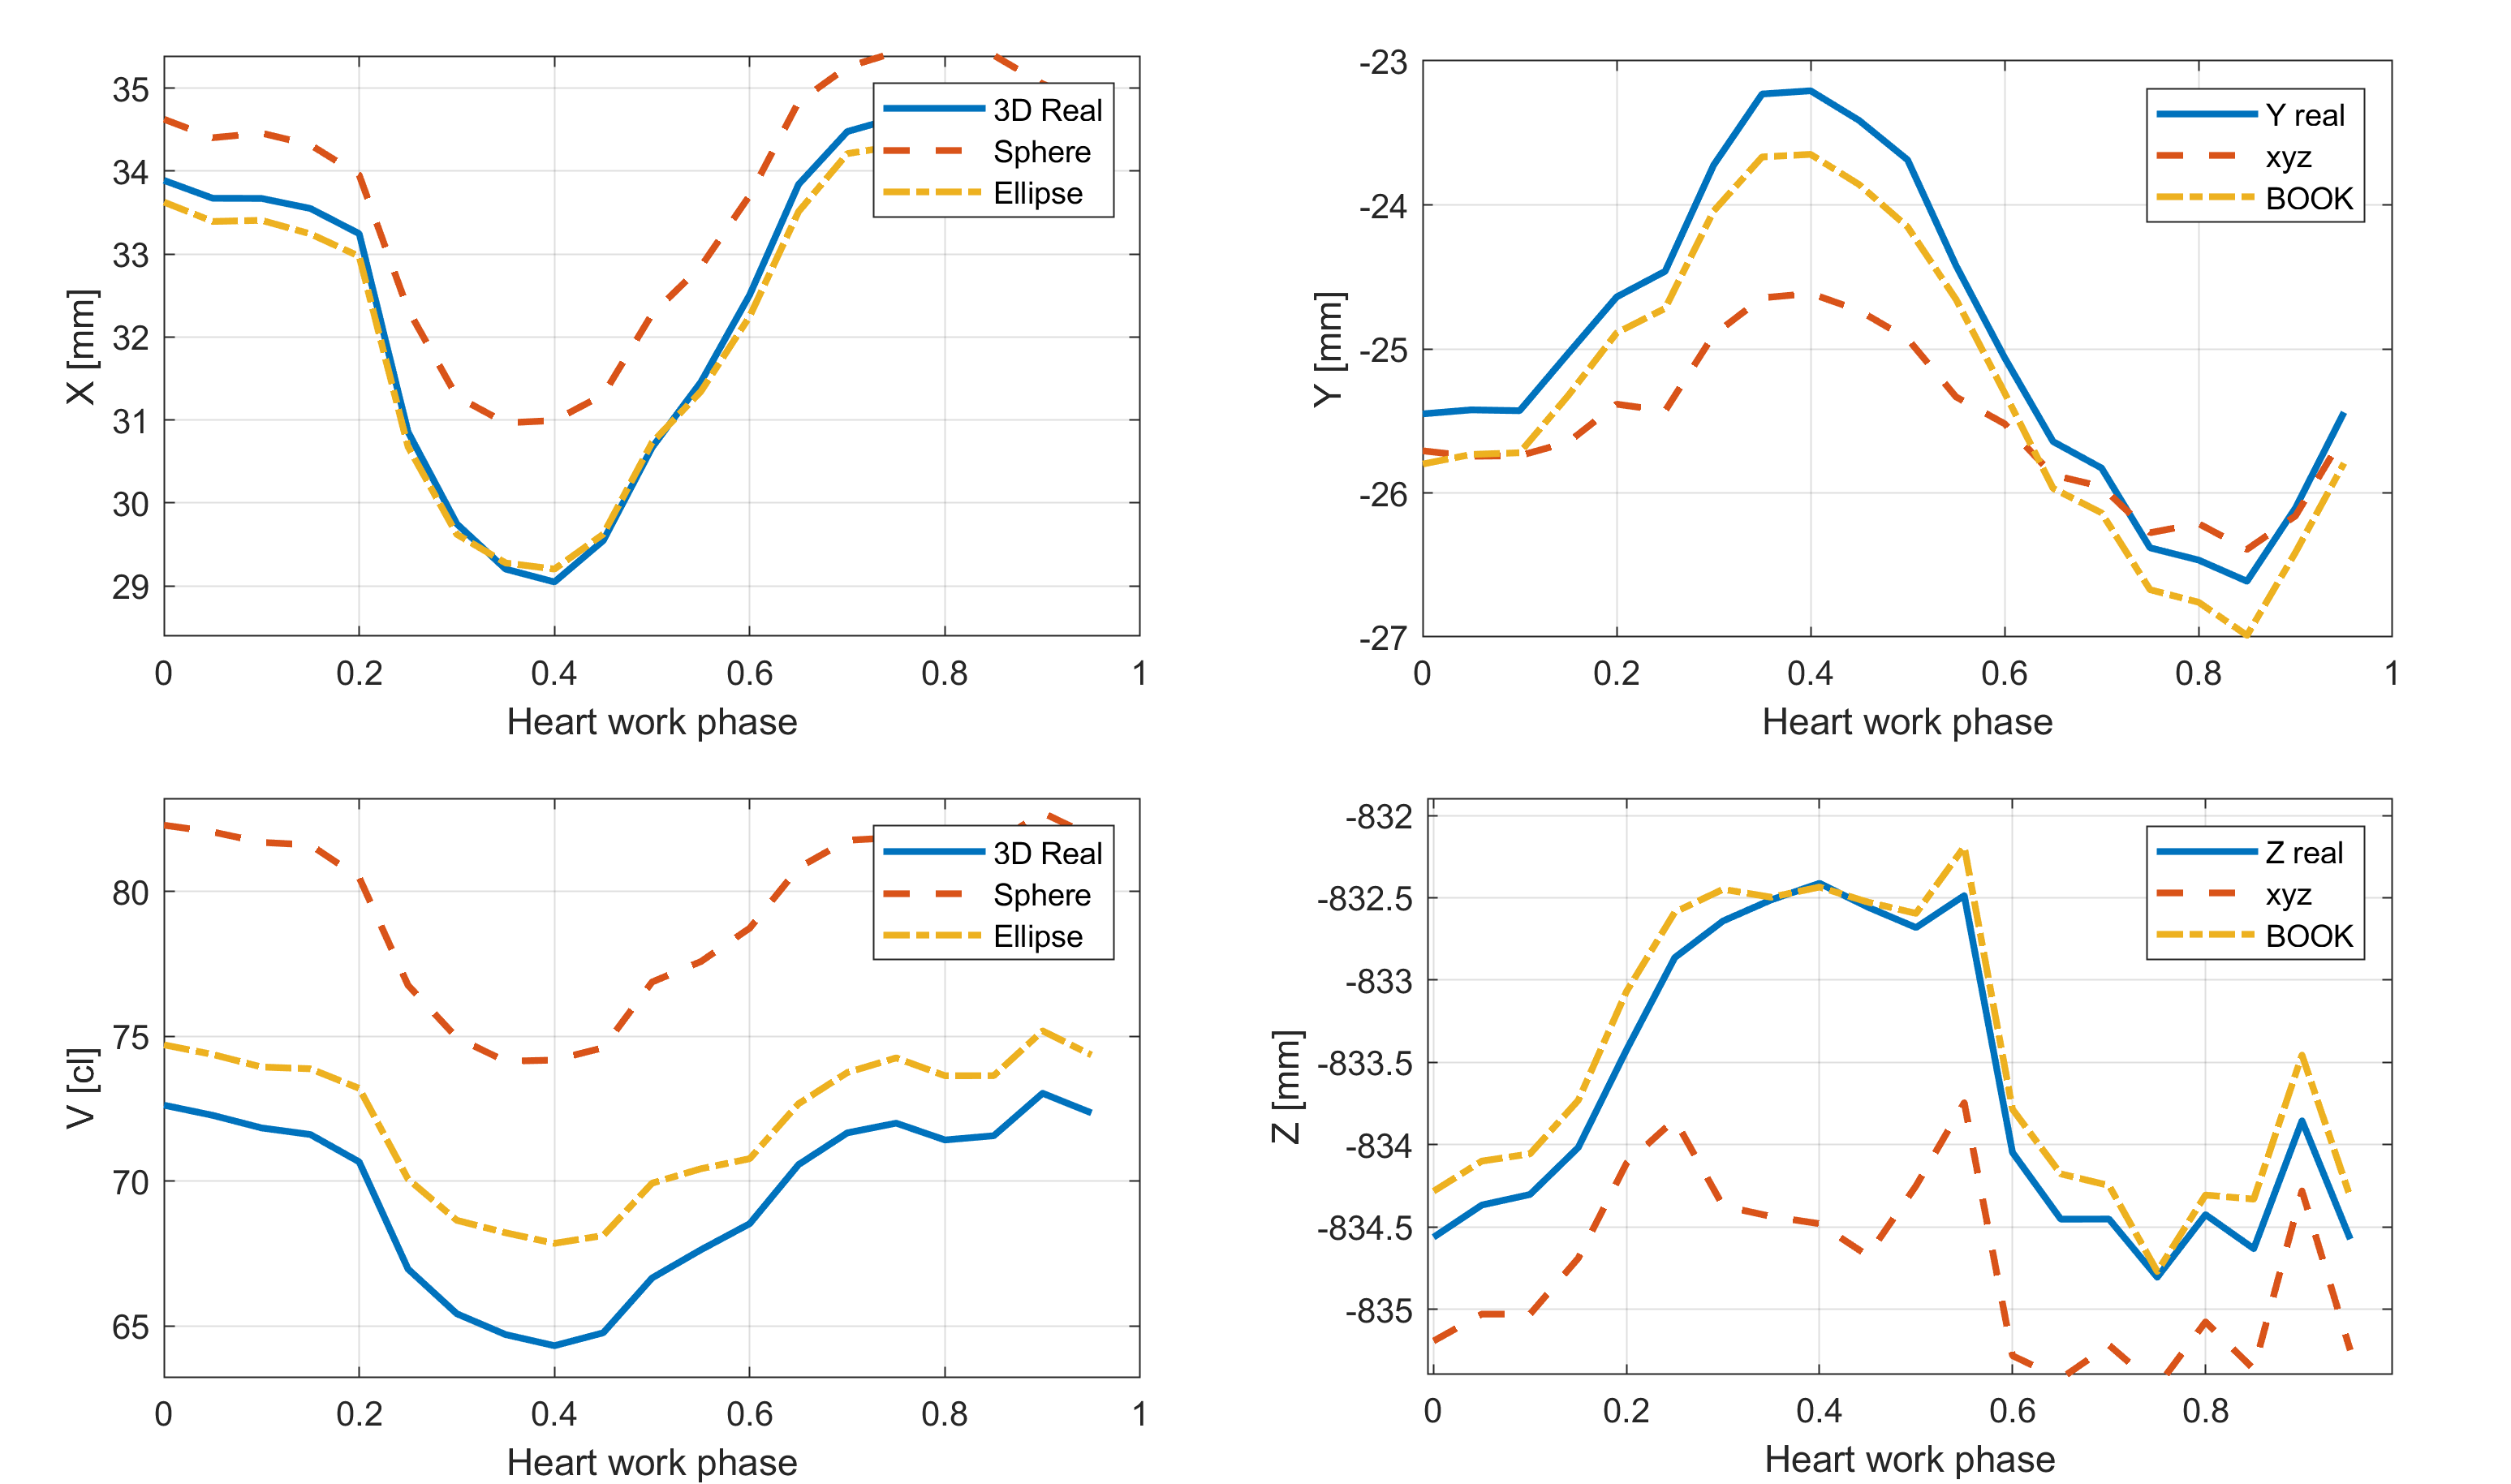
\includegraphics[width=\linewidth]{fig/1_4}
%    \caption{}
%    \label{fig:14}
%\end{figure}

In the simulation, the heart's blood is often represented as the sphere in
electrical impedance measurement problems,
%[наши статьи]
as well as in precordial mapping methods and electrical impedance tomography of
the heart. 
%[статьи по томографии]

This model is quite simple. According to the tomography data, the sphere's
parameters are determined - the radius and coordinates of the center. The
heart's contraction corresponds to a change in the radius of the sphere and
center's offset.

Using the ellipsoid model allows for a better approximation of blood in the
heart before the onset of ventricular systole. 
% статьи по эллипсу

However, the number of model parameters increases - three semiaxes of the
ellipsoid, coordinates of the center, and rotation of the ellipsoid in space
compared to one radius and the center's coordinates. The heart's contraction
corresponds to a change in the semiaxes of the ellipsoid and a shift in its
center. Also, the ellipsoid can be spatially rotated during contraction. 

The models' geometric parameters were obtained from the data of a CT of a
healthy volunteer. The study of multispiral computed tomography was carried out
in Pirogov Moscow City Clinical Hospital №1  with  Toshiba Aquilion PRIME 160
and under the patronage of employees of both the clinic and the medical center
of the BMSTU medical center. 

The study was carried out with the introduction of an iodine-containing contrast
agent Optiray 350 mg, 90 ml for the study on inspiration and 90 ml for the study
on exhalation, 50 ml at a rate of 3.5 ml/sec, and 40 ml at a rate of 3 ml/sec. 

The study was carried out on free expiration. As a result of these studies'
reconstruction, sets of slices with a time resolution of 20 series per cardio
cycle were obtained, which gives about 35-50 ms between the series. The distance
between the axial slices was 2.5 mm. The sets of sections were used to
reconstruct a 3D model of blood in the heart. 

\subsection{Sphere and Ellipsoid Approximation}
The parameters of the sphere and ellipsoid were obtained by approximating 3D models of the heart's blood.

The sphere was approximated by the criterion of the least square deviation of the sphere boundaries and real 3D geometry.

Approximation criterion \ref{eq:sphere_criteria},
$p_i$ - a finite set of points on the surface of a 3D heart model,
$dist(p_i,Z(f))$ -  distance from the point $p_i$ to the surface of the sphere $Z(f)$. 
\begin{equation}
    \sum_{i=1}^{q}dist(p_i,Z(f))^2 \rightarrow min
    \label{eq:sphere_criteria}
\end{equation}

The ellipsoid was obtained according to the criterion described in . 
%todo добавить ссылку на статью BOOK
The method is peculiar because authors consider the distance from a point to the
ellipsoid $dist(p_i, Z(f))$ as follows: the difference between 1) the
distance from the center of the ellipsoid to the point and 2) the distance from
the center of the ellipsoid to a point on its boundary. The said point is lying
on the ray outgoing their center and passing through a given point. This
assumption's error is estimated depending on the ratio of the ellipsoid
semiaxes, and an adjustment is made. The final optimization criterion is also
the least square method (2). 

Analysis of the results and visualization of the approximation showed that the
septa of the heart, such as the interventricular septum, 
%todo ссылка на рисунок модели серца
the atrioventricular septum (Fig.~\ref{fig:wall}) forms points that distort
the approximation results, causing an increase in the average deviation of the
surface of the approximating ellipse or sphere from the outer boundary of the 3D
blood model. 
%----------------------------------------------------------------------------
\begin{figure}[tbph]
    \centering
    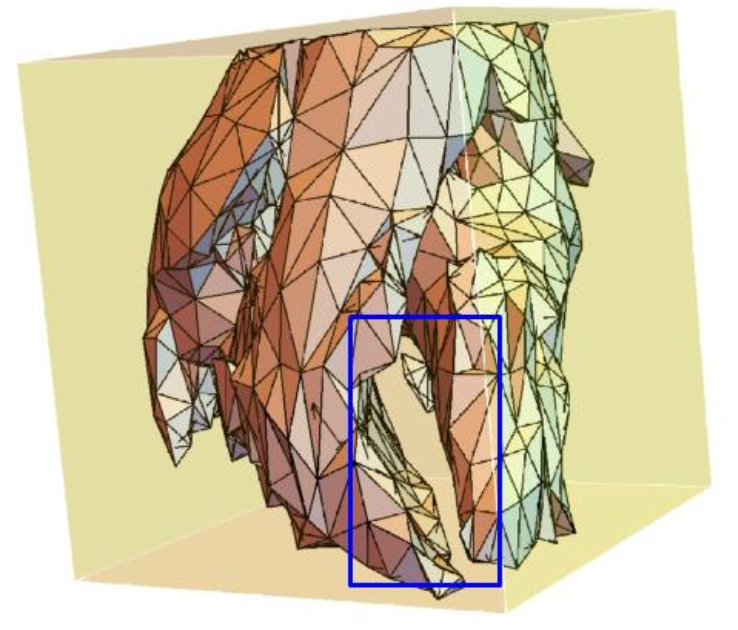
\includegraphics[width=0.8\linewidth]{fig/wall}
    \caption{3D model of blood in the heart (interventricular septum highlighted in blue)}
    \label{fig:wall}
\end{figure}
To eliminate this problem, it was decided to fill in the original 3D models of
the heart partitions and internal voids. For this, the 3D model was laid out on
2D images obtained by sectioning by planes parallel to the X and Y axes (Fig.~\ref{fig:algo}). 
%--------------------------------------------------------
\begin{figure}[tbph]
    \centering
    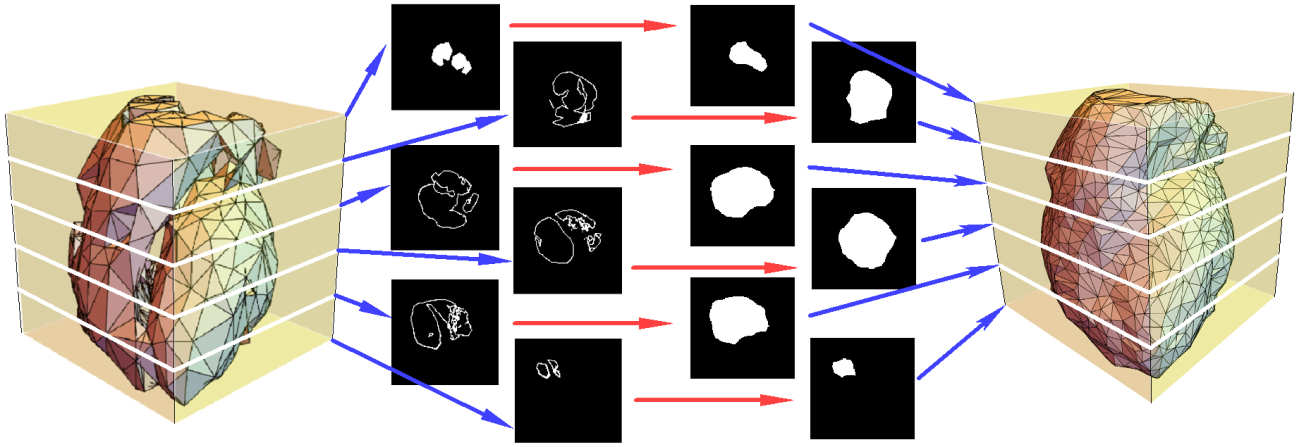
\includegraphics[width=\linewidth]{fig/algo}
    \caption{Algorithm for filling the septa of the heart in the 3D model of the heart's blood 
    (on the left - the original 3D model, on the right - the 3D model after filling the septa)}
    \label{fig:algo}
\end{figure}
%---------------------------------------------------------
Then a tangent path traversal was made of the 2D image contour with a circle radius of
20 mm (red circle), as a result of a set of obtained sections filled with septum
was going to the 3D image of the heart (Fig.~\ref{fig:algo2}).

\begin{figure}[tbph]
    \centering
    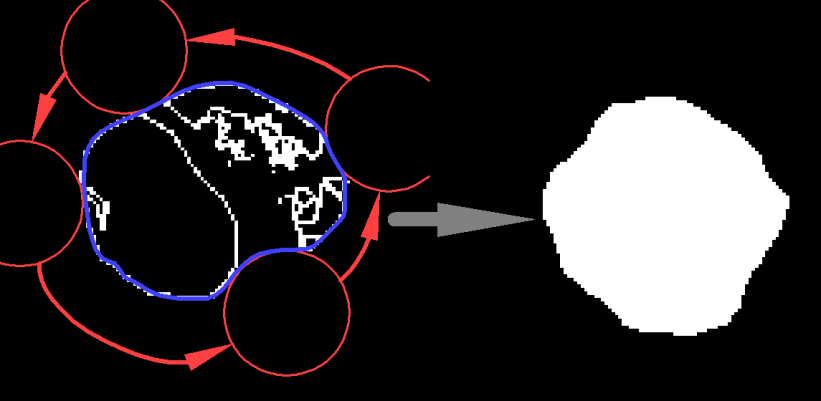
\includegraphics[width=\linewidth]{fig/algo2}
    \caption{Tangent path traversal of a 2D image with a circleto fill heart's semptum
    in the 3D models of heart's blood (on the left is white contour beforethe septum filling,
        on the right side - after the filling)}
    \label{fig:algo2}
\end{figure}

\section{Modelling}
\section{Electrical Impedance modelling parameters}
To analyze the obtained geometric models, electrical impedance modeling was
carried out in the Comsol Multiphysics CAD. The location of the electrode
systems during modeling corresponded to the location of the electrode systems
during longitudinal-transverse mapping. The distance between the current
electrodes varied from 80 to 240 mm, and the ratio of the distance between the
current electrodes to the distance between the potential ones was 2 to 1.

Values of resistivity of inclusion and homogeneous half-space are presented in
the table \ref{tab:table}.

\begin{table}[htbp]
    \caption{Resisitivity values at  100 kHz used in the model study}
    \begin{center}
        \begin{tabular}{|l|c|c|}
            \hline
            \multirow{2}{*}{\textbf{Tissue}}              &     \textbf{Resistivity values,}      &    \textbf{Resistivity value in}  \\
            &    \Omega \cdot \textbf{m}     &   \textbf{ simulation, } \Omega \cdot \textbf{m }\\
            \hline
            Blood (Hct=50)           & 1.35 [21]           & 1.35      \\
            \hline
            Myocardium               & 4.6 [20]       & \multirow{7}{*}{4.2}\\
            \cline{1-2}
            \multirow{2}{*}{Muscles} & 2.7 [20]          &     \\
            \cline{2-2}
            & 1.5 – 25 [19]           &   \\
            \cline{1-2}
            Lung (deflated)          & 3.68 [20]     &         \\
            \cline{1-2}
            Lung                     & 1.6 – 10 [1]       &    \\
            \cline{1-2}
            Human thorax & \multirow{2}{*}{4.63 [19]}  &   \\
            (average)   & &   \\
            \hline
        \end{tabular}
        \label{tab:table}
    \end{center}
\end{table}
%todo поправить список литературы в таблице

The averaging of the specific resistances of the lung, muscle tissue, and
myocardium is possible since measurements are considered in the phase of calm
expiration, and the specific resistance of the lung tissue on expiration
approaches the specific resistance of muscle tissue. 

\subsection{Comparison of the 3D model with sphere and ellipsoid}

Several parameters were used to compare the models themselves and the results of
modeling the real 3D geometry of blood in the heart, sphere, and ellipsoid.
First, a comparison of the change in the volume of blood in the heart  was made.
the volume of a real 3D model was compared with the volumes of the approximating
sphere and ellipsoid. The volumes were estimated for each of the 20 points when
the cardio cycle was split. Second, the movement of blood volume in the heart as
a whole was considered, i.e. the movement of the center of mass of a real 3D
model and its approximating figures. Third, the electrical impedance change
dependencies during the cardiac cycle were compared for different positions and
sizes of electrode systems.

\begin{figure}[htbp]
%    \centerline{
\includegraphics{fig/fig1.png}}
    \centering{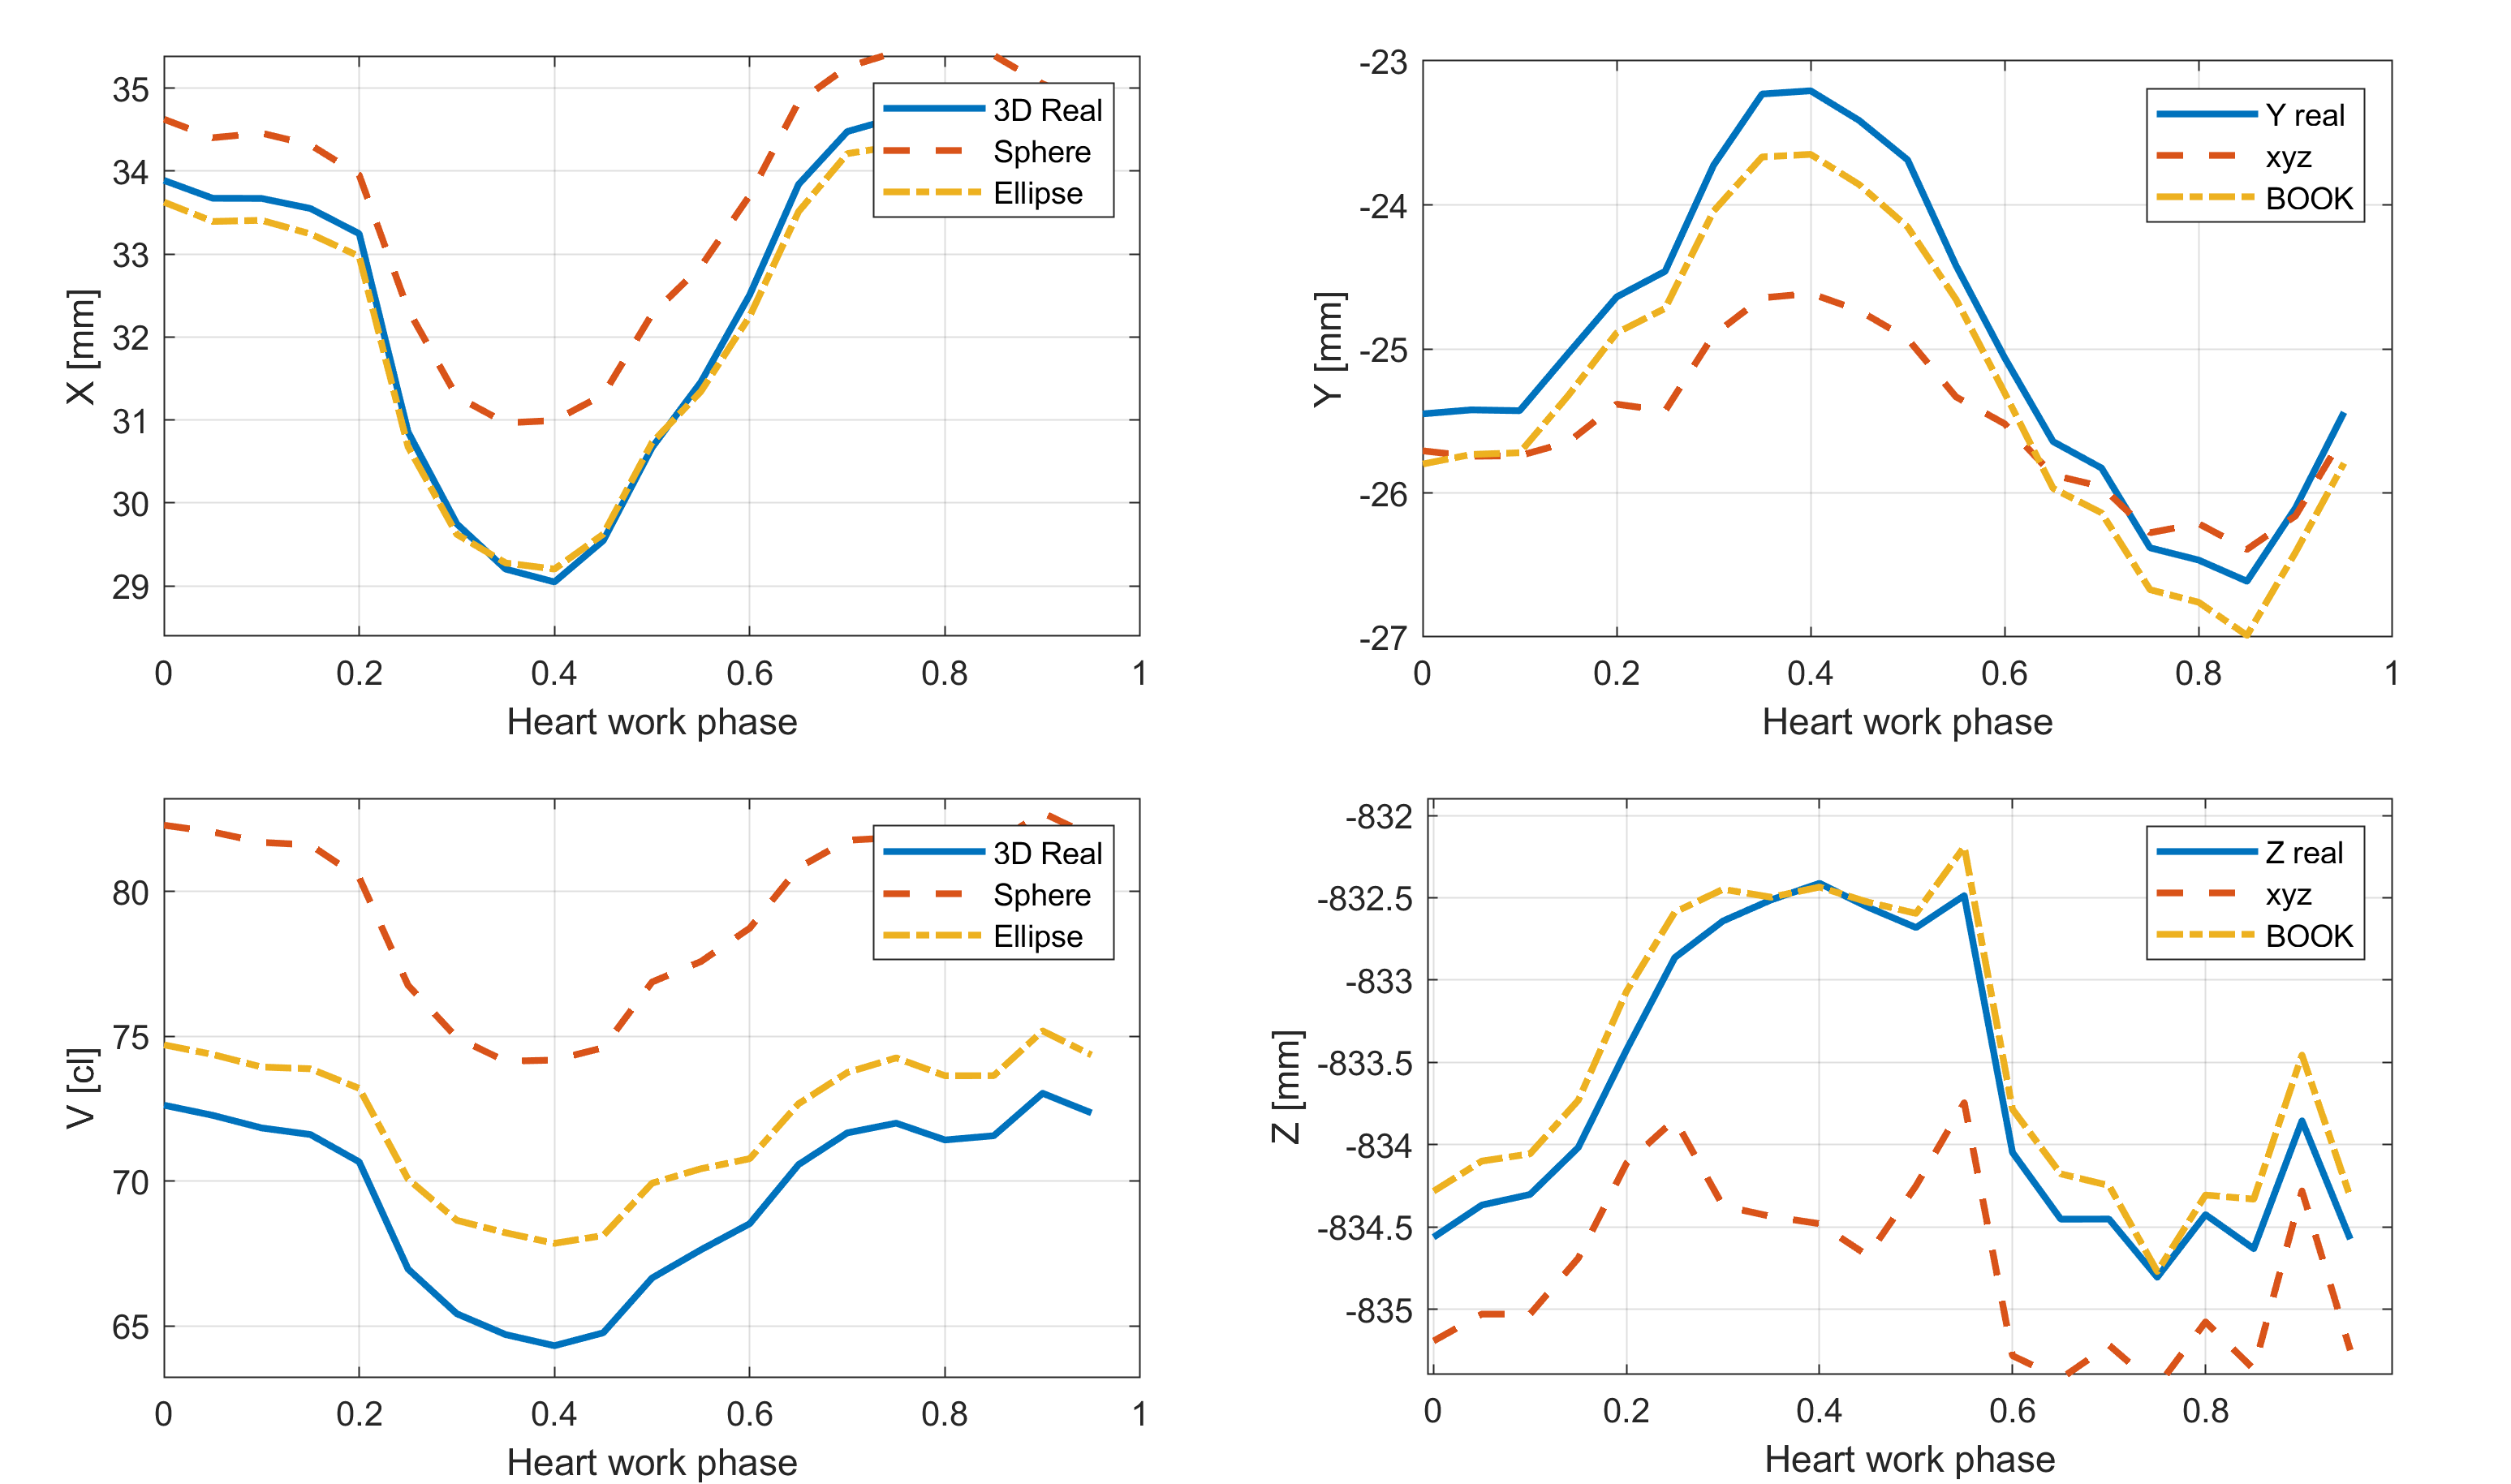
\includegraphics[width=\linewidth]{fig/1_4}}
    \caption{Change during the cardiac cycle of the coordinates of the center of mass (X, Y, Z) and volume of the original 3D model, sphere and ellipsoid}
    \label{fig:rxyz}
\end{figure}

\section{Results}

The dependences of the change in the volume and coordinates of the center of
mass of the original 3D model, and the sphere and ellipsoid are shown in
Fig.~\ref{fig:rxyz}, where the t-axis is R-to-R interval of cardiac cycle. 
% по оси абсцисс

The simulation results of impedance changes during the cardiac cycle are
presented in Fig. ~\ref{real}, Fig.~\ref{fig:sphere}, Fig.~\ref{fig:ellipse}.
For each model, dependences are presented for the electrode system located along
the heart's anatomical axis and perpendicular to it. These graphs also consider
the cardiac cycle from R-wave to R-wave. 

\begin{figure}[tbph]
    \centering
    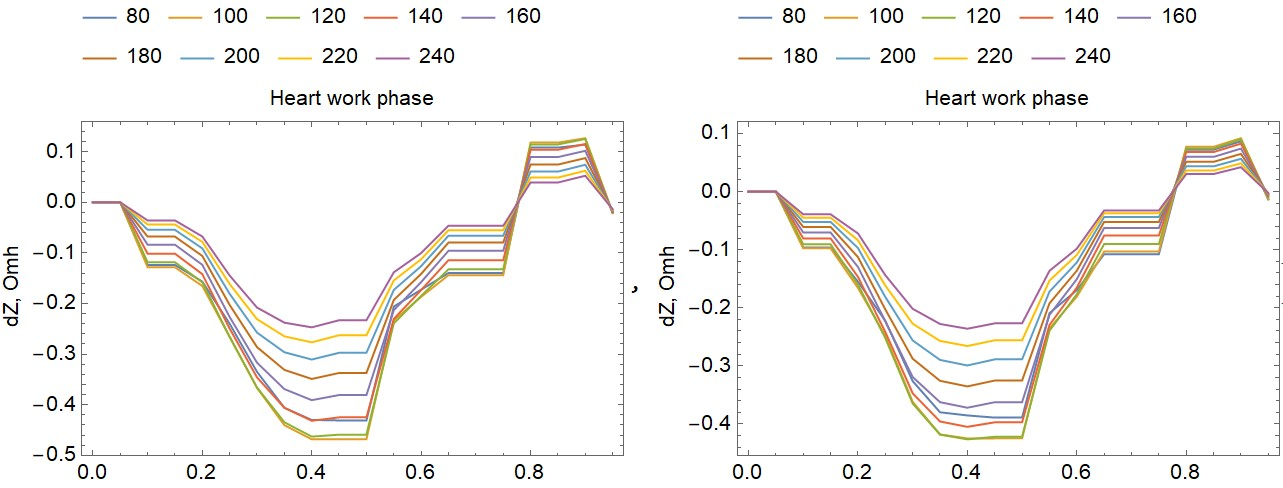
\includegraphics[width=\linewidth]{fig/real}
    \caption{Dependence of electrical impedance changes during the cardiac cycle for the initial 3D model (location of the electrode system along the heart axis - to the left, perpendicular to the heart axis - to the right)}
    \label{real}
\end{figure}

\begin{figure}[tbph]
    \centering
    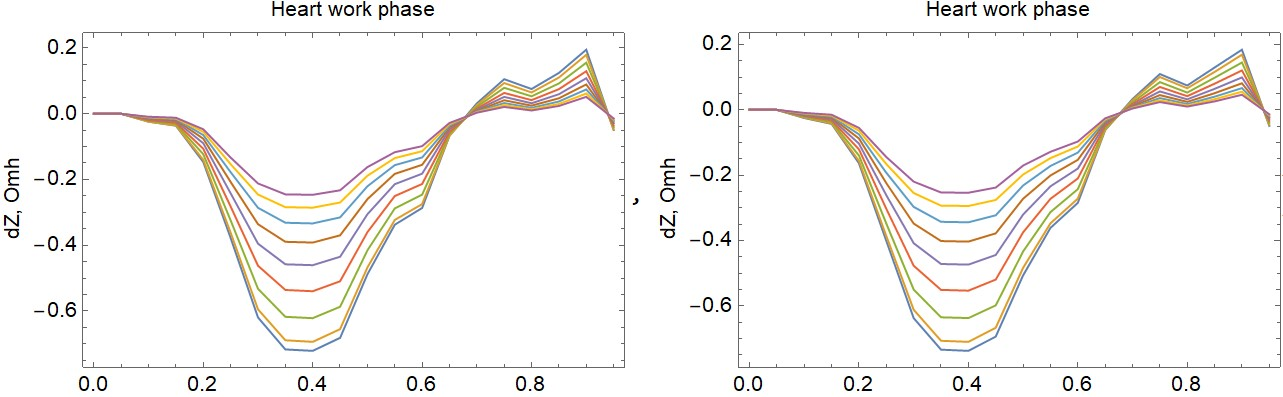
\includegraphics[width=\linewidth]{fig/sphere}
    \caption{Dependence of electrical impedance changes during the cardiac cycle for a spherical model (the location of the electrode system along the heart axis - to the left, perpendicular to the heart axis - to the right)}
    \label{fig:sphere}
\end{figure}

\begin{figure}[tbph]
    \centering
    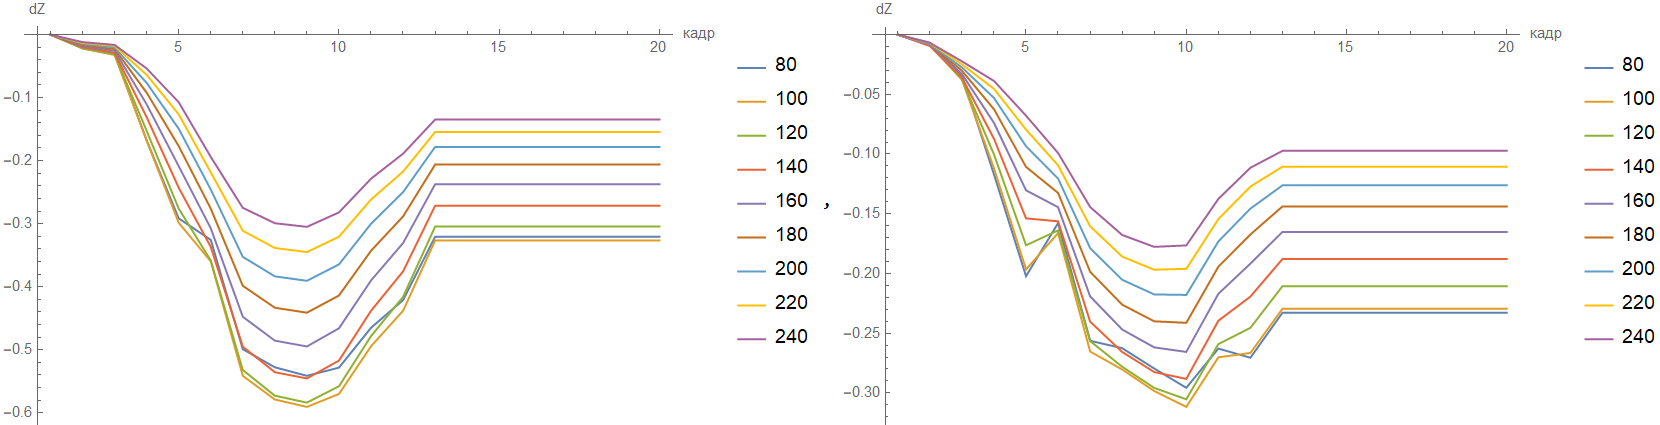
\includegraphics[width=\linewidth]{ellipse}
    \caption{Dependence of electrical impedance changes during the cardiac cycle for an elliptical model (the location of the electrode system along the heart axis - on the left, perpendicular to the heart axis - on the right)}
    \label{fig:ellipse}
\end{figure}

\section{Discussion}

When comparing the motion of the center of mass of the original 3D model and the
approximating sphere and ellipsoid from Fig. \ref{fig:rxyz} it is seen that the
center of mass of the ellipsoid moves in accordance with the center of mass of
the 3D model. The sphere's movement qualitatively corresponds to the movement of
the 3D model, but quantitatively it differs - less amplitude. The ellipsoid
volume differs by an average of 3-5\% during the cardiac cycle; for a sphere,
the difference reaches 12-15\%. This effect can influence and introduce
additional errors in assessing hemodynamic characteristics based on the sphere's
geometric model.

The waveforms of the electrical impedance modeling signal for the sphere and the
ellipsoid qualitatively correspond to the initial 3D model waveform but differ
significantly in amplitude characteristics. For a numerical assessment of the
obtained simulation results, the value of the impedance change during
ventricular systole $ \Delta Z $ was compared. The difference in values ​​in
Fig.\ref{real} at the time points corresponds to 0\% and 40\% of the cardiac
cycle (beginning and end of ventricular systole). For small electrode systems
(80-120 mm), $\Delta Z$ for a 3D model differs by \% from $\Delta Z $ for a
sphere and \% from $\Delta Z$ for an ellipsoid. For large electrode systems
(200-240 mm), $\Delta Z$ for a 3D model differs by \% from $\Delta Z$ for a
sphere and \% from $\Delta Z $ for an ellipsoid.%todo заполнить проценты

\section{Conclusion}

Studies have shown that for a given volunteer, an elliptical geometric model of
the heart's blood approximates the heart's real 3D geometry with an error of
3-5\% and is preferable when assessing hemodynamic parameters. Simultaneously,
electrical impedance modeling showed that when using electrode systems 80-120 mm
in size, it is preferable to use an elliptical geometric model, and when using
large electrode systems 200-240 mm, it is preferable to use a spherical
geometric model. Since electrode systems with sizes over 180 mm are usually used
for precordial longitudinal-transverse mapping, it is necessary to use a
spherical mathematical model.

The conclusions are valid for this volunteer. At the moment, studies are
underway on three more healthy volunteers to evaluate the findings. 
%An excellent style manual for science writers is \cite{b7}.

\begin{thebibliography}{00}
\bibitem{b1} G. Eason, B. Noble, and I. N. Sneddon, ``On certain integrals of Lipschitz-Hankel type involving products of Bessel functions,'' Phil. Trans. Roy. Soc. London, vol. A247, pp. 529--551, April 1955.
\bibitem{b2} J. Clerk Maxwell, A Treatise on Electricity and Magnetism, 3rd ed., vol. 2. Oxford: Clarendon, 1892, pp.68--73.
\bibitem{b3} I. S. Jacobs and C. P. Bean, ``Fine particles, thin films and exchange anisotropy,'' in Magnetism, vol. III, G. T. Rado and H. Suhl, Eds. New York: Academic, 1963, pp. 271--350.
\bibitem{b4} K. Elissa, ``Title of paper if known,'' unpublished.
\bibitem{b5} R. Nicole, ``Title of paper with only first word capitalized,'' J. Name Stand. Abbrev., in press.
\bibitem{b6} Y. Yorozu, M. Hirano, K. Oka, and Y. Tagawa, ``Electron spectroscopy studies on magneto-optical media and plastic substrate interface,'' IEEE Transl. J. Magn. Japan, vol. 2, pp. 740--741, August 1987 [Digests 9th Annual Conf. Magnetics Japan, p. 301, 1982].
\bibitem{b7} M. Young, The Technical Writer's Handbook. Mill Valley, CA: University Science, 1989.
\end{thebibliography}
\vspace{12pt}
%\color{red}
%IEEE conference templates contain guidance text for composing and formatting conference papers. Please ensure that all template text is removed from your conference paper prior to submission to the conference. Failure to remove the template text from your paper may result in your paper not being published.

\end{document}
